\section{Преимущества и недостатки систем IOT}
\subsection{Преимущества}
Преимущества IoT охватывают все сферы жизни и бизнеса. Вот список некоторых из
преимуществ, которые может предложить IoT:
\begin{itemize}
    \item Улучшение взаимодействия с клиентами. Текущая аналитика страдает от «слепых зон» и
          существенные недостатки в точности и, как уже отмечалось, взаимодействие с такими системами остается пассивным. Интернет вещей полностью
          трансформирует это, чтобы добиться более богатого и эффективного взаимодействия с аудиторией. Применение концпеции IOT в современном мире показано на рисунке \ref{fig:section3:iot}.

          \begin
          {figure}[h!]
          \centering
          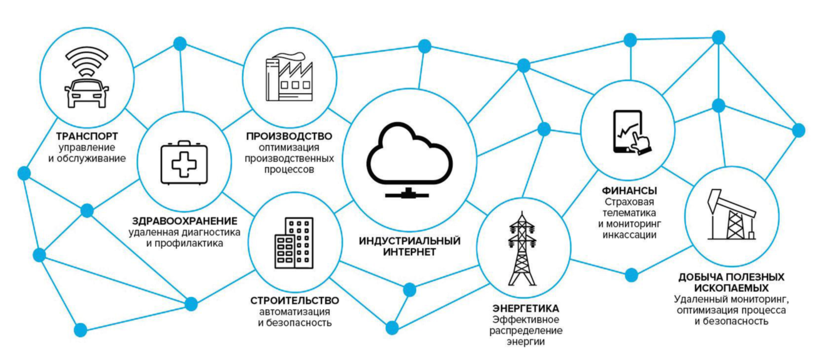
\includegraphics[scale=1]{iot.png}
          \caption{Применение концепции IoT}
          \label{fig:section3:iot}
          \end{figure}

    \item Оптимизация технологий – Те же технологии и данные, которые улучшают
          пользовательский опыт также улучшает использование устройств и помогает в более эффективных улучшениях
          технологии IoT. Интернет вещей открывает мир важных функциональных и полевых данных.
    \item Сокращение отходов – IoT делает очевидными области улучшений. Текущая аналитика без использования рассматриваемой концепции дает нам
          поверхностное понимание, а IoT предоставляет реальную информацию, что ведет к более эффективному
          управлению ресурсами.
    \item  Усовершенствованный сбор данных. Современный сбор данных имеет свои ограничения и
          основывается на пассивном их использовании. IoT вырывает его из этих пространств и размещает именно там, где
          люди действительно хотят видеть проанализованные данные, чтобы проанализировать происходящее в их окружении. Это позволяет получить более полную картину всего.
\end{itemize}
\subsection{Недостатки}
Хотя IoT обеспечивает впечатляющий набор преимуществ, он также сопряжен со значительным набором проблем.
Вот список некоторых его основных проблем:
\begin{itemize}
    \item Безопасность – IoT создает экосистему постоянно подключенных устройств, обменивающихся данными по сети.
          Система предлагает мало контроля над обменом трафика, несмотря на любые меры безопасности. Это оставляет
          пользователей подверженными разными видами атак.
    \item Конфиденциальность — изощренность IoT позволяет предоставлять существенные личные данные в мельчайших подробностях,
          без уведомления пользователя об этой процедуре.
    \item Сложность. Некоторые считают системы IoT сложными с точки зрения проектирования, развертывания и
          техническое обслуживание, учитывая их использование нескольких технологий и большого набора новых возможностей
          технологии. На рисунке \ref{fig:section3:arch} приведен пример архитектры базовой системы IoT.

          \begin
          {figure}[h!]
          \centering
          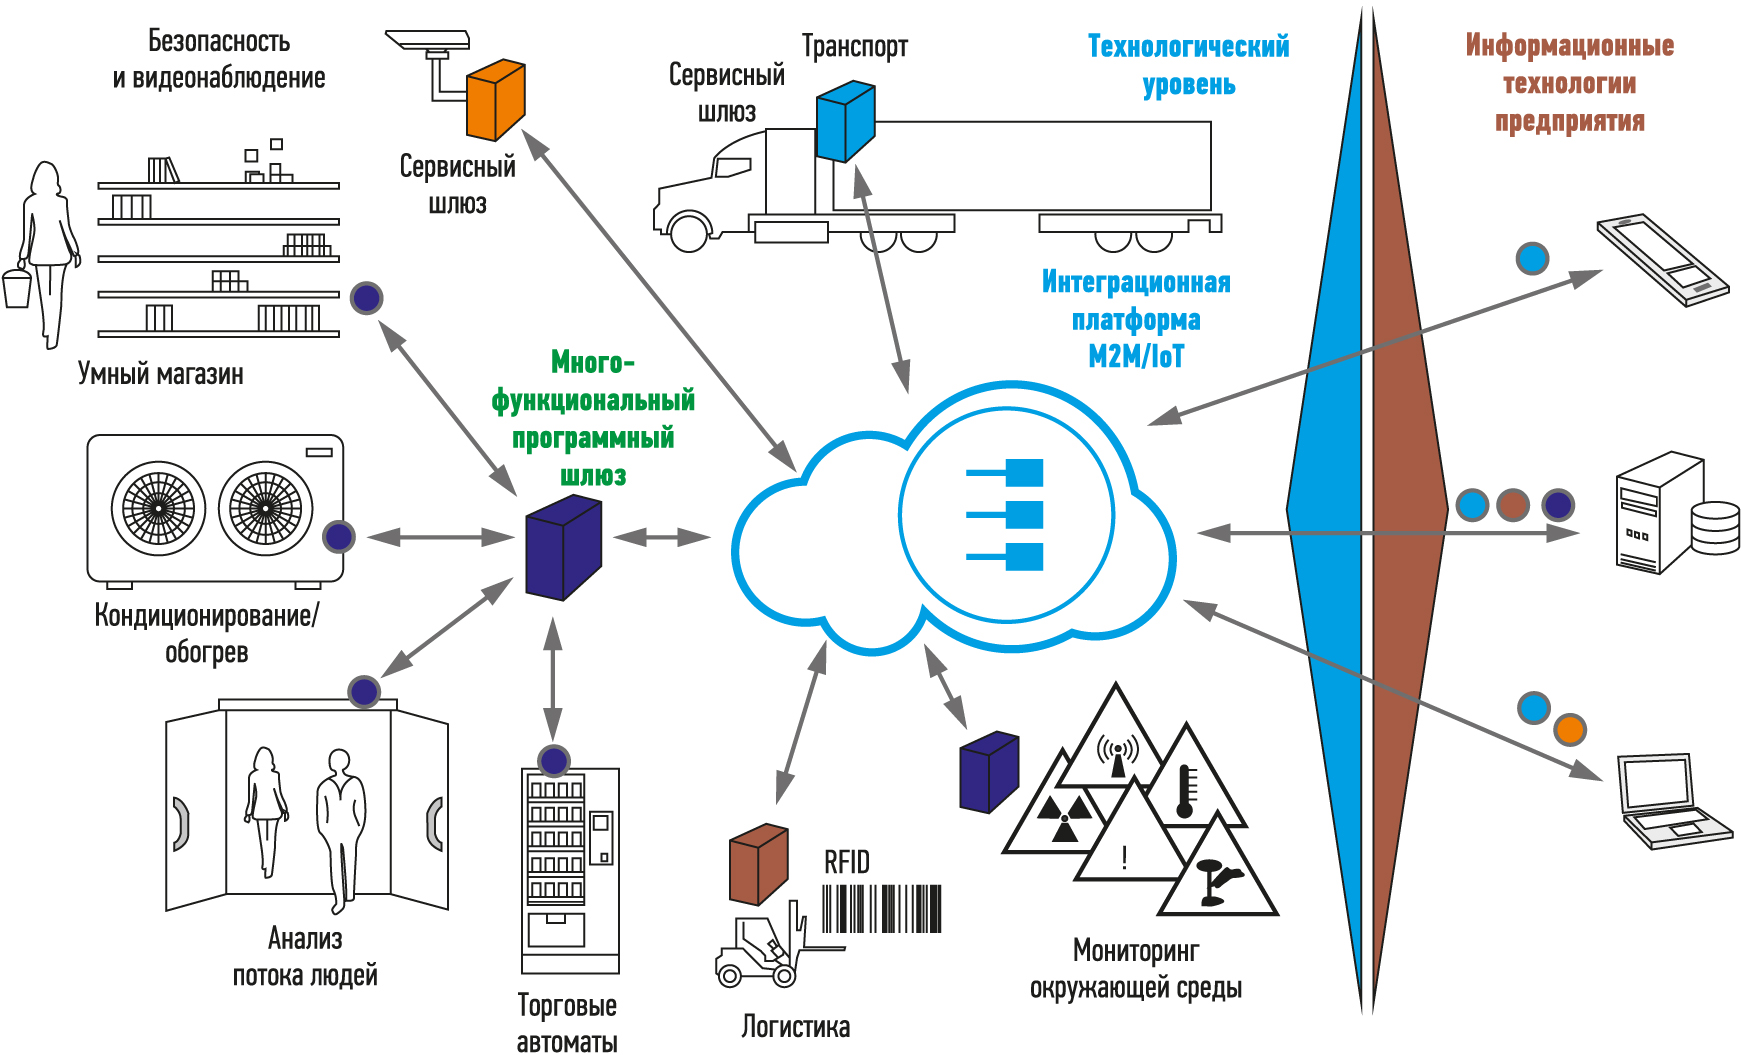
\includegraphics[scale=1]{arch.jpg}
          \caption{Пример архитектуры системы IoT}
          \label{fig:section3:arch}
          \end{figure}
\end{itemize}